\documentclass[xcolor=dvipsnames]{beamer}
\usecolortheme[named=Brown]{structure}
\usetheme{Malmoe}
\useoutertheme{infolines}
% All the information about beamer themes comes from here
% http://en.wikibooks.org/wiki/LaTeX/Presentations

\usepackage{ross}
\DeclareMathOperator{\Real}{Re}
\DeclareMathOperator{\Imag}{Im}
\DeclareMathOperator{\Mat}{Mat}
\usepackage{tikz}
\usetikzlibrary{calc}
% \usepackage{pgfplots}
% \pgfplotsset{width=7cm,compat=1.8}
\usepackage{standalone}

\setbeamertemplate{footline}[frame number]{} 

\usepackage{framed,color}
\definecolor{shadecolor}{HTML}{ffddcc}


%Information for the title slide
\title{Moduli Space of Harmonic Tori in $S^3$}
\author{Ross Ogilvie}
\institute[]{
  School of Mathematics and Statistics\\
  University of Sydney
  }
\date{June 2017}

% This puts a table of contents showing where you are up to at the start of every section
% \AtBeginSection[]
% {
%   \begin{frame}
%     \frametitle{Table of Contents}
%     \tableofcontents[currentsection]
%   \end{frame}
% }

%gets rid of navigation symbols, which are stupid
\setbeamertemplate{navigation symbols}{}

%%%%%%%%%%%%%%%%%
% Document starts
%%%%%%%%%%%%%%%%%
\begin{document}
\begin{frame}
    \titlepage
\end{frame}


\begin{frame}{Harmonic Map}
\begin{itemize}
\item Let $f : T^2 \to S^3 = SU(2)$ be a harmonic map.
\item A harmonic map is a critical point of the energy functional. 
\item Long historical interest in minimal and constant curvature surfaces. A surface is CMC iff its Gauss map is harmonic.
\item Minimal surfaces = conformal harmonic = CMC with zero mean curvature.
\item Thought to be quite rare; Hopf Conjecture. Wente (1984) constructed immersed CMC tori.
\item A classification of such maps is given by spectral data $(Σ,Θ,\tilde{Θ},E)$ (Hitchin, Pinkall-Sterling, Bobenko).
\end{itemize}
\end{frame}


\begin{frame}{Spectral Data $(Σ,Θ,\tilde{Θ},E)$}
\begin{itemize}
\item Spectral curve $Σ$ is a real (possibly singular) hyperelliptic curve,
\begin{align*}
η^2 = \prod (ζ-α_i)(1-\bar{α}_i ζ)
\end{align*}
\item $Θ,\tilde{Θ}$ are differentials with double poles and no residues over $ζ=0,\infty$. 
\item Period conditions: The periods of $Θ,\tilde{Θ}$ must lie in $2π\iu \Z$.
\item Closing conditions: for $γ_+$ a path in $Σ$ between the two points over $ζ=1$, and $γ_-$ between the points over $ζ=-1$ then
\[
\int_{γ_+} Θ , \int_{γ_-} Θ, \int_{γ_+} \tilde{Θ} , \int_{γ_-} \tilde{Θ} \in 2π\iu\Z.
\]
\item $E$ is a quaternionic line bundle of a certain degree.
\end{itemize}
\end{frame}


% \begin{frame}{CMC Spectral Data}
% \begin{itemize}
% \item Compatible spectral curve construction. Very similar conditions. 
% \item Spectral curve is branched over $ζ=0,\infty$.
% \item Same symmetry and periodicity conditions on differentials $Θ$ and $\tilde{Θ}$.
% \item Closing conditions apply over points $ζ=1,λ$ for some $λ\in \S^1$.

% \end{itemize}
% \end{frame}


\begin{frame}{CMC Moduli Space (Kilian-Schmidt-Schmitt)}
\begin{itemize}
% \item It is natural to use the spectral data to ask deformation and moduli space questions.
\item One can vary the line bundle $E$, so called isospectral deformations.
\item CMC non-isospectral deformations. Maps come in one dimensional families.
\item $\mathcal{M}^{CMC}_0$ is disjoint lines parametrised by $H\in\R$~\\
\begin{center}
\includestandalone[width=0.4\textwidth]{graphics/cmc_low_moduli}
\end{center}
\item Components $\mathcal{M}^{CMC}_1$ end in either $\mathcal{M}^{CMC}_0$ or bouquet of spheres.
\end{itemize}
\end{frame}


\begin{frame}{Harmonic Map Example}
\begin{itemize}
\begin{shaded}
\item 
$f(x+\iu y) = \exp(-4x\mathbf{X})\exp(4y\mathbf{Y})$, for
\[
\mathbf{X} = \begin{pmatrix} 0 & 1 \\ -1 & 0 \end{pmatrix},\qquad
\mathbf{Y} = \begin{pmatrix} 0 & δ \\ -δ & 0 \end{pmatrix},\qquad
\Im δ > 0
\]
\end{shaded}
\item 
This map is periodic. Formula well-defined on any torus $\C/Γ$, where $Γ$ is a sublattice of this periodicity lattice.
\begin{center}
\includestandalone[width=0.4\textwidth]{graphics/genus_zero_lattice}
\end{center}
\end{itemize}
\end{frame}


\begin{frame}
\begin{itemize}
\item Holding either $x$ or $y$ constant gives circles.
\item As $δ\to \R^\times$, image collapses to a circle.
\item As $δ\to 0,\infty$, the periodicity lattice degenerates.
\begin{center}
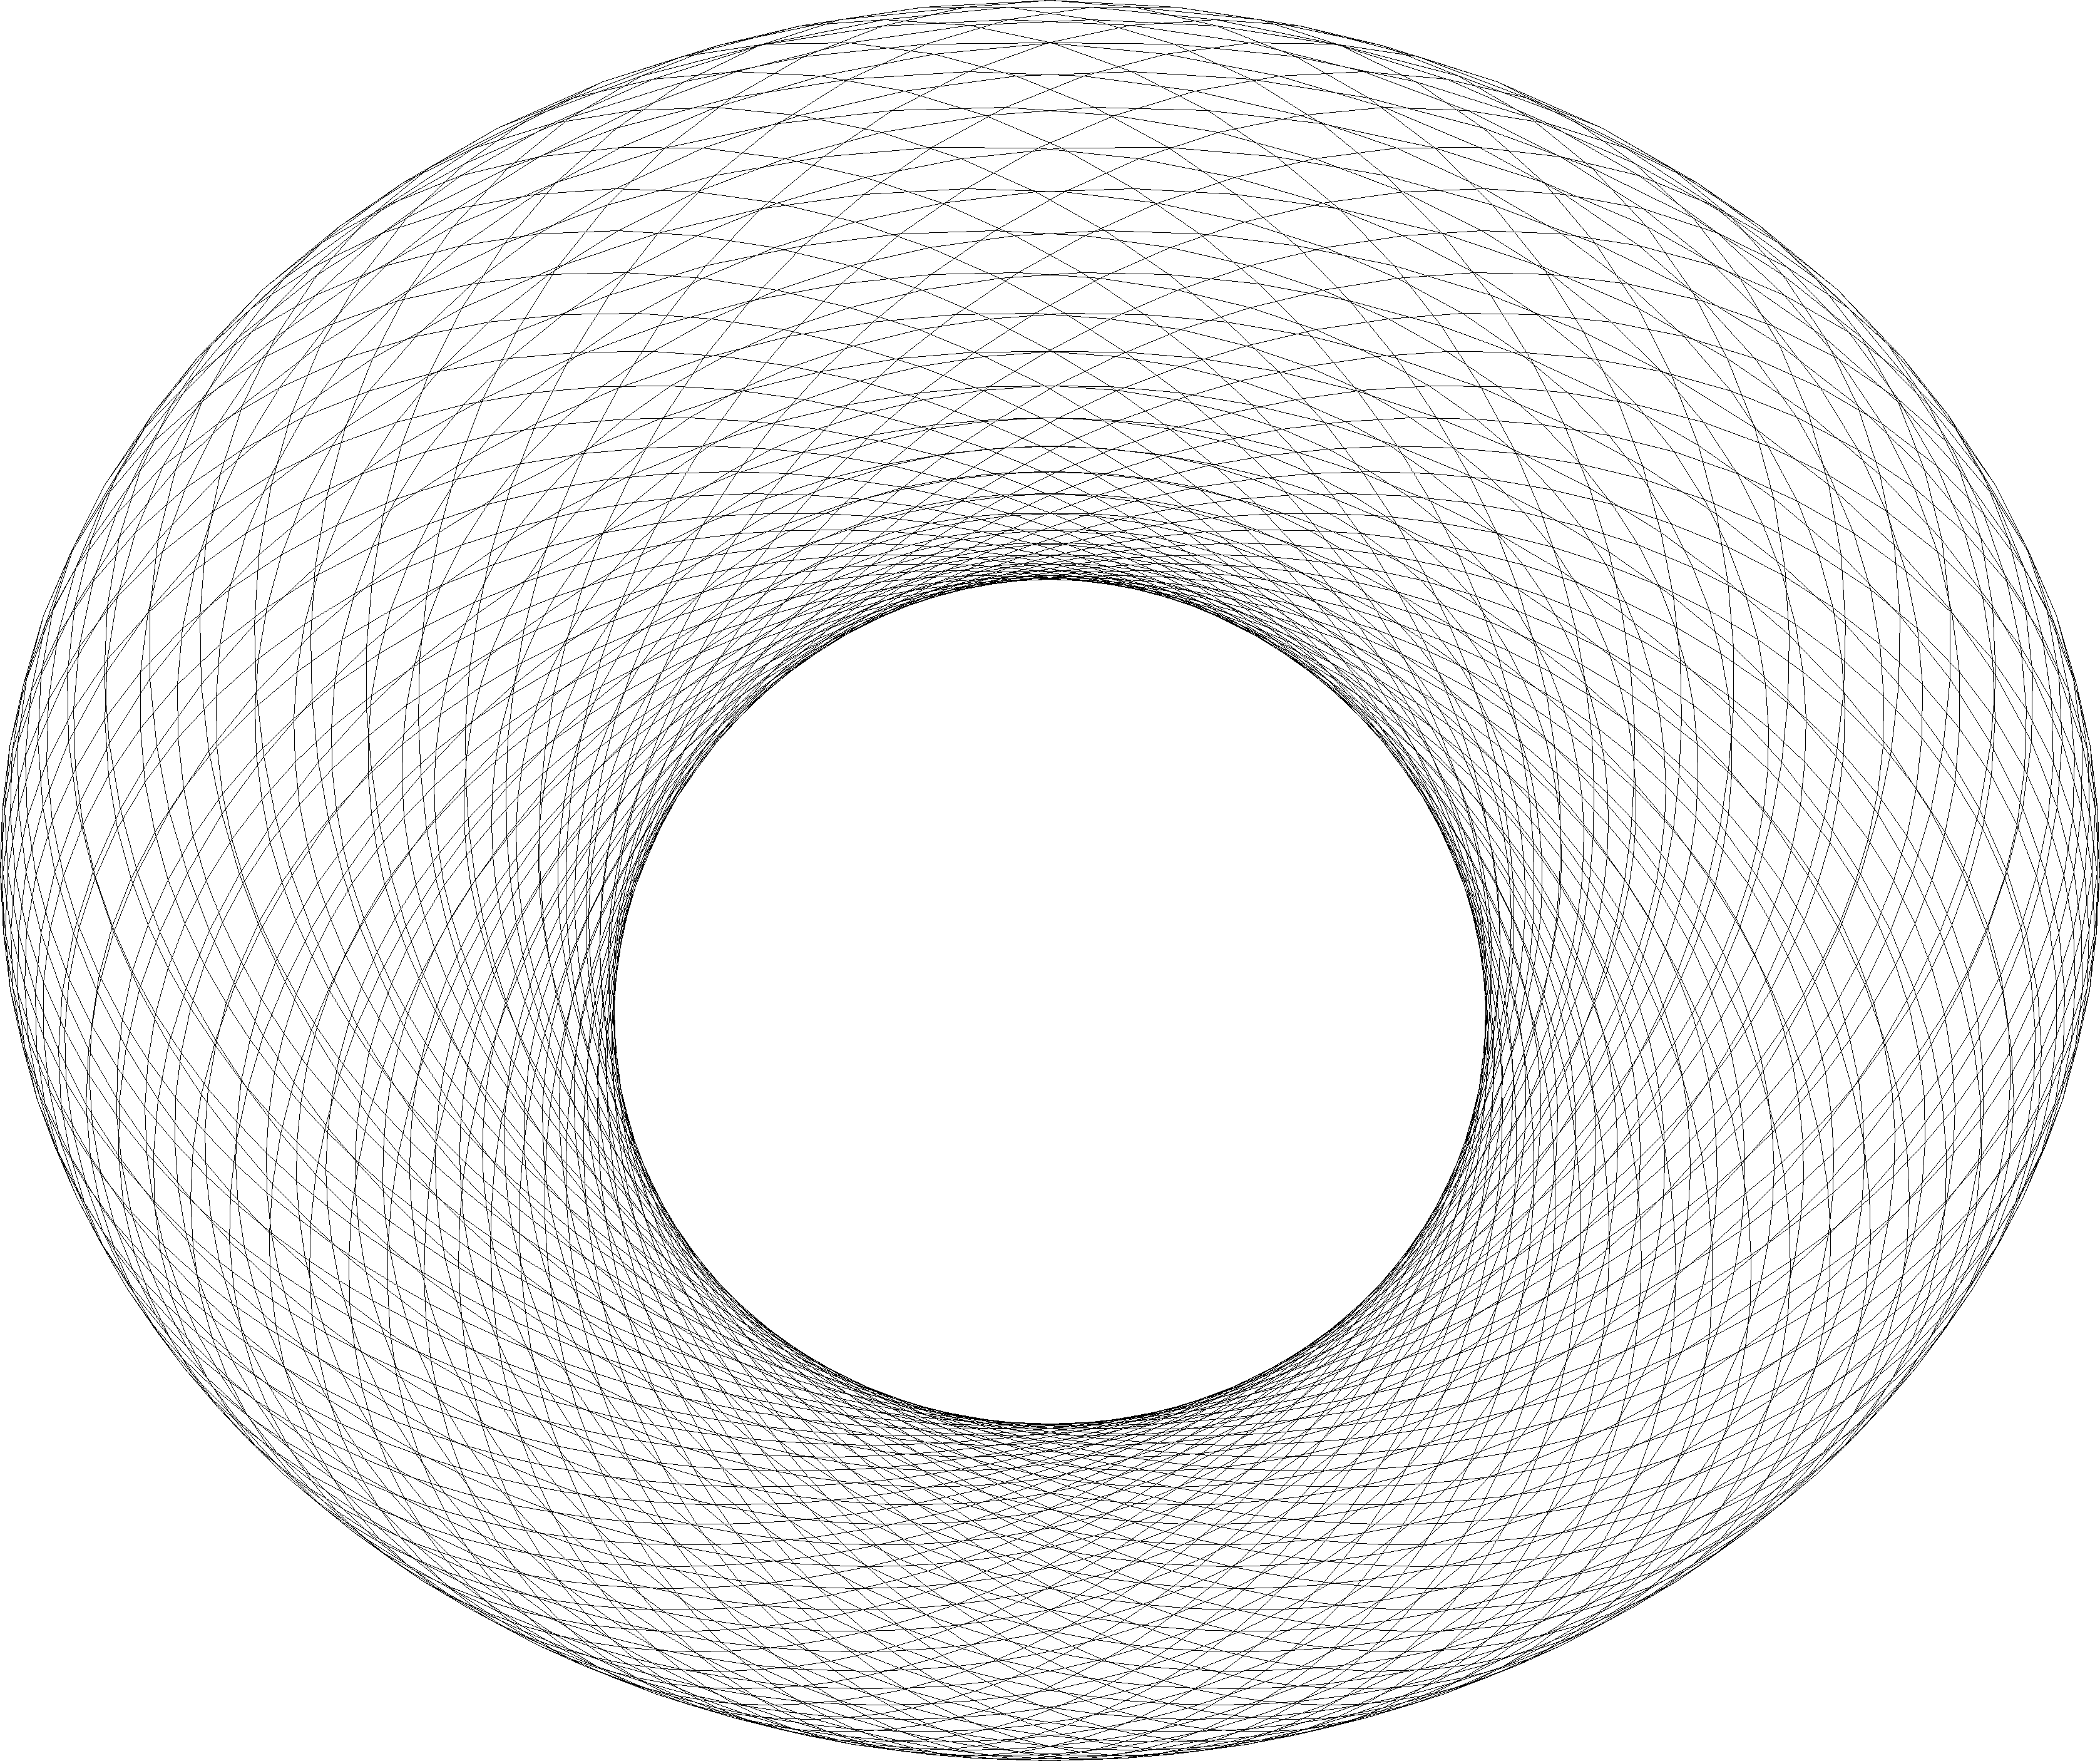
\includegraphics[height=40mm]{graphics/genus0_plot_pi4.png}
\hspace{1cm}
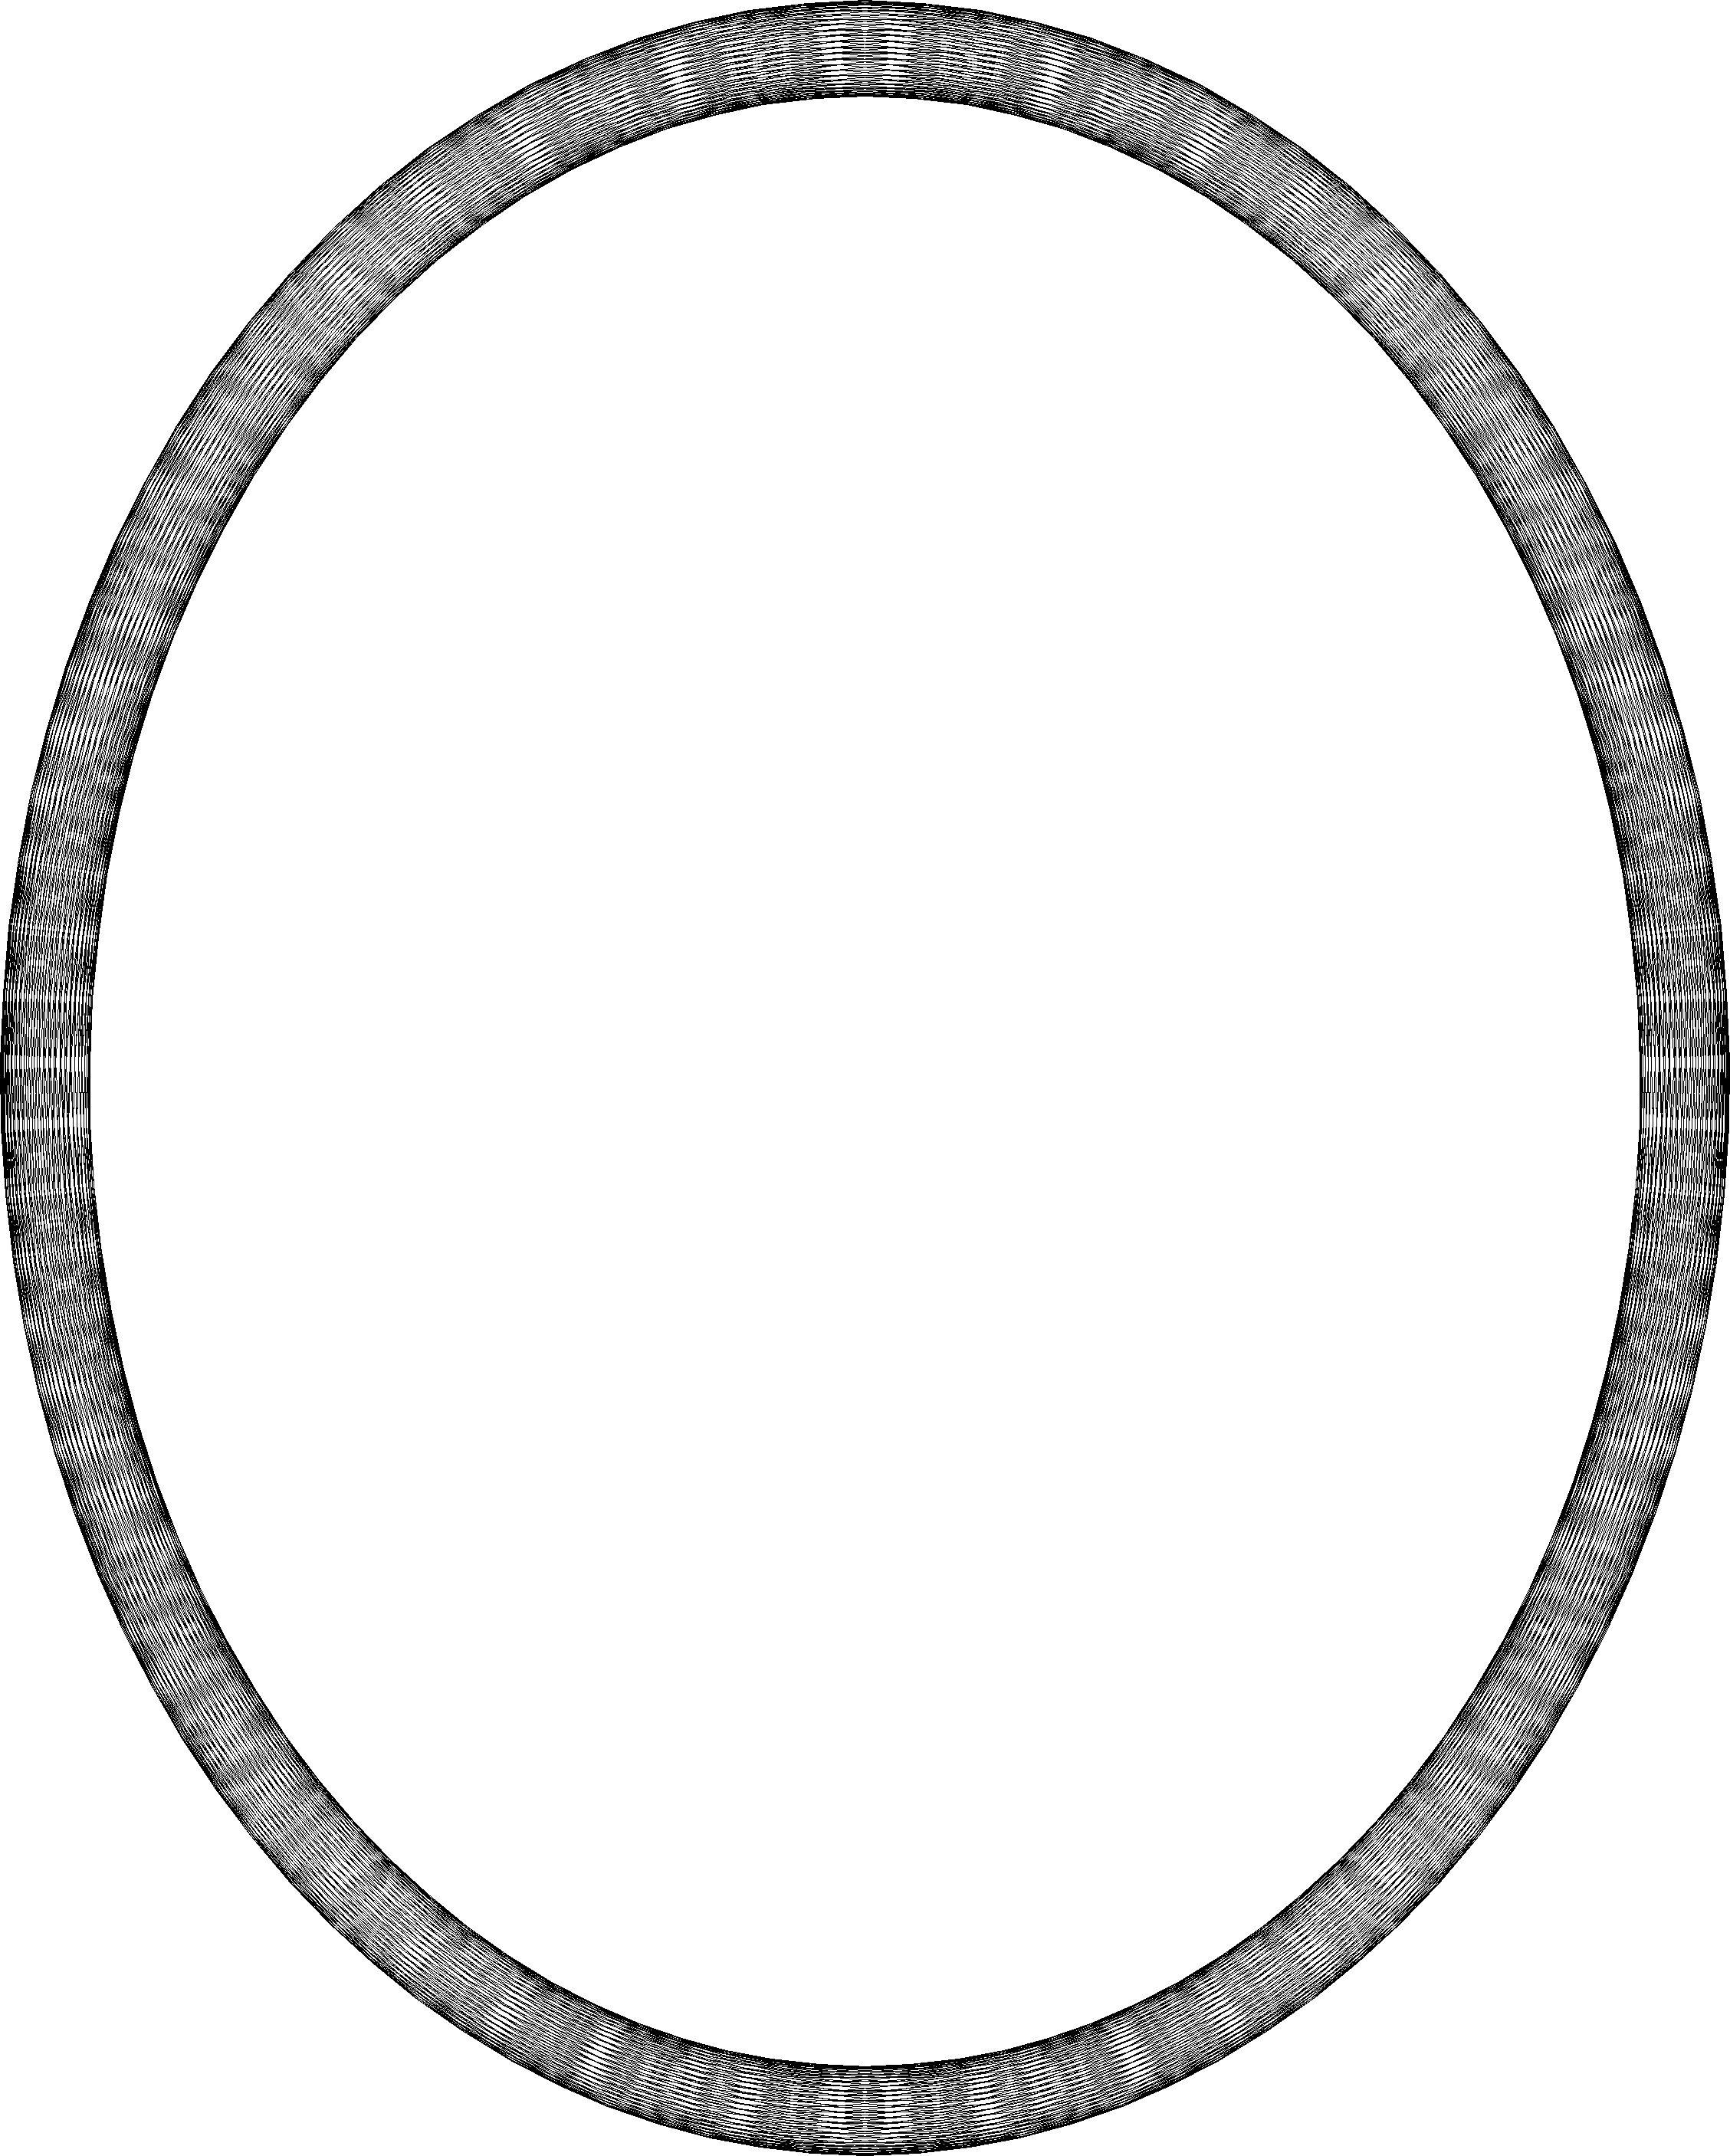
\includegraphics[height=40mm]{graphics/genus0_plot_pi32.png}
\end{center}
\end{itemize}
\end{frame}


\begin{frame}{Constructing Spectral Data}
\begin{itemize}
\item Up to translations, $f$ is determined by the Lie algebra valued map $f^{-1}df$, the pullback of the Mauer-Cartan form. 
\item Decompose into its $dz$ and $d\bar{z}$ parts $f^{-1} df = 2(Φ - Φ^*)$.
\item Use $f$ to pull pack the Levi-Civita connection on $SU(2)$ to get a connection $A$.
\item Given a pair $(Φ,A)$, we can make a family of flat $SL(2,\C)$ connections. Let $ζ\in\C^\times$ be the \emph{spectral parameter} and define
\[
d_ζ := d_A + ζ^{-1}Φ - ζ Φ^*
\]
\end{itemize}
\begin{shaded}
Family of connections is
\begin{align*}
d_ζ 
= d &- \left[ (\mathbf{X}-\iu \mathbf{Y}) + ζ^{-1} (\mathbf{X}+\iu \mathbf{Y}) \right] dz \\
&\quad - \left[ (\mathbf{X}+\iu \mathbf{Y}) + ζ (\mathbf{X}-\iu \mathbf{Y}) \right] d\bar{z} \\
= d &- ζ^{-1}\left[ (\mathbf{X}+\iu \mathbf{Y}) + ζ (\mathbf{X}-\iu \mathbf{Y}) \right]\left[ dz + ζ d\bar{z}\right]
\end{align*}
\end{shaded}
\end{frame}


\begin{frame}{Holonomy}
\begin{itemize}
\item Because the connections are flat, we can define holonomy for them. 
\item Pick a base point and generators for the fundamental group, ie take two loops around the torus.
\item Parallel translating vectors with $d_ζ$ around one loop gives a linear map on the tangent space at the base point. Call this $H(ζ)$. Around the other loop call the transformation $\tilde H(ζ)$.
\begin{shaded}
\begin{align*}
H_τ(ζ) &= \exp \left\{ ζ^{-1}\left[ (\mathbf{X}+\iu \mathbf{Y}) + ζ (\mathbf{X}-\iu \mathbf{Y}) \right]\left[ τ + ζ \bar{τ}\right] \right\}
\end{align*}
\end{shaded}
\end{itemize}
\end{frame}


\begin{frame}{Spectral curve}
\begin{itemize}
\item The fundamental group of $T^2$ is abelian, so $H$ and $\tilde{H}$ commute. Therefore they have common eigenspaces.
\item Define
\[
Σ = \text{closure } \left\{ (ζ, L) \in \C^\times \times \CP^1 \mid L \text{ is an eigenline for } H(ζ) \right\}
\]
\item The eigenvalues of $H(ζ)$ are $μ(ζ), μ(ζ)^{-1}$. The characteristic polynomial is
\[
μ^2 - (\tr H) μ + 1 = 0
\]
\item Using the compactness of the torus, one can show that $(\tr H)^2 - 4$ vanishes to odd order only finitely many times. The spectral curve is always finite genus for harmonic maps $T^2 \to \S^3$.
\end{itemize}
\end{frame}


\begin{frame}
\begin{itemize}
\begin{shaded}
\item From example
\[
Σ = \left\{ \left(ζ, \left[\pm \sqrt{(1-\iu δ)(ζ-α)}:\sqrt{-(1+\iu \bar{δ})(1-\bar{α}ζ)} \right]\right) \right\}  
\]
for
\[
α = \frac{1+\iu δ}{-1 + \iu δ} 
\qquad\Leftrightarrow\qquad
δ = \iu \frac{1+α}{1 - α}  
\]
\item
Can write equation for $Σ$ as
\begin{align*}
η^2 &= (ζ-α)(1-\bar{α}ζ)
\end{align*}
\end{shaded}
\end{itemize}
\end{frame}




\begin{frame}{The Differentials}
\begin{itemize}
\item The differentials come from the eigenvalues $μ(ζ), \tilde{μ}(ζ)$ of $H(ζ),\tilde{H}(ζ)$. These functions have essential singularities.
\item However $\log μ, \log \tilde {μ}$ are holomorphic on $\C^\times$ and have simple poles above $ζ=0,\infty$.
\item $d \log μ$ removes the additive ambiguity of $\log$. Thus we set 
$Θ = d \log μ$ and $\tilde {Θ} = d \log \tilde {μ}$
\item In order to recover the eigenvalues, one requires residue free double poles over $ζ=0,\infty$ and that the periods of the differentials lie in $2π\iu\Z$.
\end{itemize}
\end{frame}


\begin{frame}
\begin{itemize}
\begin{shaded}
\item The eigenvalues of $H_τ(ζ)$ are
\begin{align*}
μ_τ(ζ,η) = \exp \left[ \iu\abs{1-\iu δ}(τ + \bar{τ}ζ)ηζ^{-1} \right].
\end{align*}
\item The corresponding differential is therefore
\begin{align*}
Θ_τ = \iu\abs{1-\iu δ}\,d\left[ (τ + \bar{τ}ζ)ηζ^{-1} \right].
\end{align*}
\end{shaded}
\item On any given spectral curve, there is a lattice of differentials that may be used in spectral data. Different choices corresponds to coverings of the same image.
\end{itemize}
\end{frame}


\begin{frame}{Moduli Space $\mathcal{M}_0$}
\begin{itemize}
\item Every spectral curve in genus zero arises from this class of examples.
\item Choice amounts to branch point $α \in D^2$ and choice of pair of differentials from a lattice
\begin{align*}
  \mathcal{M}_0 &= \coprod D^2
\end{align*}
\item Image degenerates: $δ \to \R^\times \quad\Leftrightarrow\quad α \to \S^1\setminus\{\pm 1\}$.
\item Lattice degenerates: $δ \to 0, \infty \quad\Leftrightarrow\quad α \to \pm 1$.
\item Two dimensional (in contrast to CMC case).
\end{itemize}
\end{frame}


\begin{frame}{Moduli Space $\mathcal{M}_g$}
\begin{theorem}
At a point $(Σ,Θ^1,Θ^2) \in \mathcal{M}_g$ corresponding to a nonconformal harmonic map, if $Σ$ is nonsingular, and $Θ^1$ and $Θ^2$ vanish simultaneously at most four times on $Σ$ and never at a ramification point of $Σ$, then $\mathcal{M}_g$ is a two-dimensional manifold in a neighbourhood of this point.
\end{theorem}
\begin{theorem}
At a point $(Σ,Θ^1,Θ^2) \in \mathcal{M}_g$ corresponding to a conformal harmonic map, if $Σ$ is nonsingular, and $Θ^1$ and $Θ^2$ never vanish simultaneously on $Σ$ then $\mathcal{M}_g$ is a two-dimensional manifold in a neighbourhood of this point.
\end{theorem}
\begin{itemize}
\item Proof uses Whitham deformations. 
% Spectral curve and differentials are written in a standard way as polynomials, embedding $\mathcal{M}_g$ in the space of polynomials. Linear equations are formulated for the tangent vectors to $\mathcal{M}_g$. The implicit function theorem is used to show local smoothness.
\end{itemize}
% $Σ$ of genus $g$ curve can be described by
% \begin{align*}
% η^2 &= P(ζ) = P_0 + P_1 ζ + \cdots + \bar{P}_1 ζ^{2g+1} + \bar{P}_0 ζ^{2g+2}
% \end{align*}
% \item A differential with the correct symmetries and poles must be of the form
% \[
% Θ = \frac{dζ}{ζ^2η} b(ζ)
% \]
% for some polynomial $b(ζ)$ of degree $g+3$. 
% \item 
\end{frame}

\begin{frame}{Genus One}
\begin{itemize}
\item Spectral curves have two pairs of branch points $α,β,\cji{α},\cji{β}$. Let $\mathcal{A}_1 = \left\{ (α,β)\in D^2\times D^2 \mid α \neq β \right\}$.
\item Not every spectral curve has differentials that meet all the conditions.
\item There is always an exact differential $Θ^E$ that meets all conditions except closing condition.
\item A multiple of $Θ^E$ meets the closing condition if and only if
\begin{align*}
S(α,β) := \frac{\abs{1-α}\abs{1-β}}{\abs{1+α}\abs{1+β}} \in \Q^+
\end{align*} 
\end{itemize}
\end{frame}

\begin{frame}
\begin{itemize}
\item Fix a value of $p\in\Q^+$. Let $\mathcal{A}_1(p) = S^{-1}(p)$. It is an open three-ball with a line removed.
\begin{center}
\begin{tikzpicture}
\draw[thick] (4,0) arc (10:170:4cm and 2cm);
\draw[thick] (4,0) arc (-10:-170:4cm and 2cm);
\draw[thick, dashed] (4,0) arc (10:170:4cm and 0.5cm);
\draw[thick] (4,0) arc (-10:-170:4cm and 0.5cm);
\draw (1.4,1.5) -- (-1.4,-1.5);
\fill (1.4,1.5) circle (0.05);
\fill (-1.4,-1.5) circle (0.05);
\end{tikzpicture}
\end{center}
\item Rugby football shaped. Ends are $(α,β) = (1,-1), (-1,1)$. Seams are points with both $α,β$ in $\S^1$.
\end{itemize}
\end{frame}


\begin{frame}
\begin{itemize}
\item There is a second differential $Θ^P$ with periods $0$ and $2π\iu$. Every differential that meets period conditions is a combination $\R Θ^E + \Z Θ^P$.
\item Define $T$, up to periods of $Θ^P$, by 
\begin{align*}
2π\iu T := p\int_{γ_-} Θ^P - \int_{γ_+} Θ^P
\end{align*}
\item A curve admits spectral data if and only if both $S\in \Q^+$ and $T \in \Q$ (and the latter is well-defined).
\item The connected components of the space of spectral curves are annuli if $S=1$ and strips $(0,1)\times\R$ if $S\neq 1$.
\item The connected components of the space of spectral data $\mathcal{M}_1$ are all strips $(0,1)\times\R$.
\end{itemize}
\end{frame}

\begin{frame}
\begin{center}
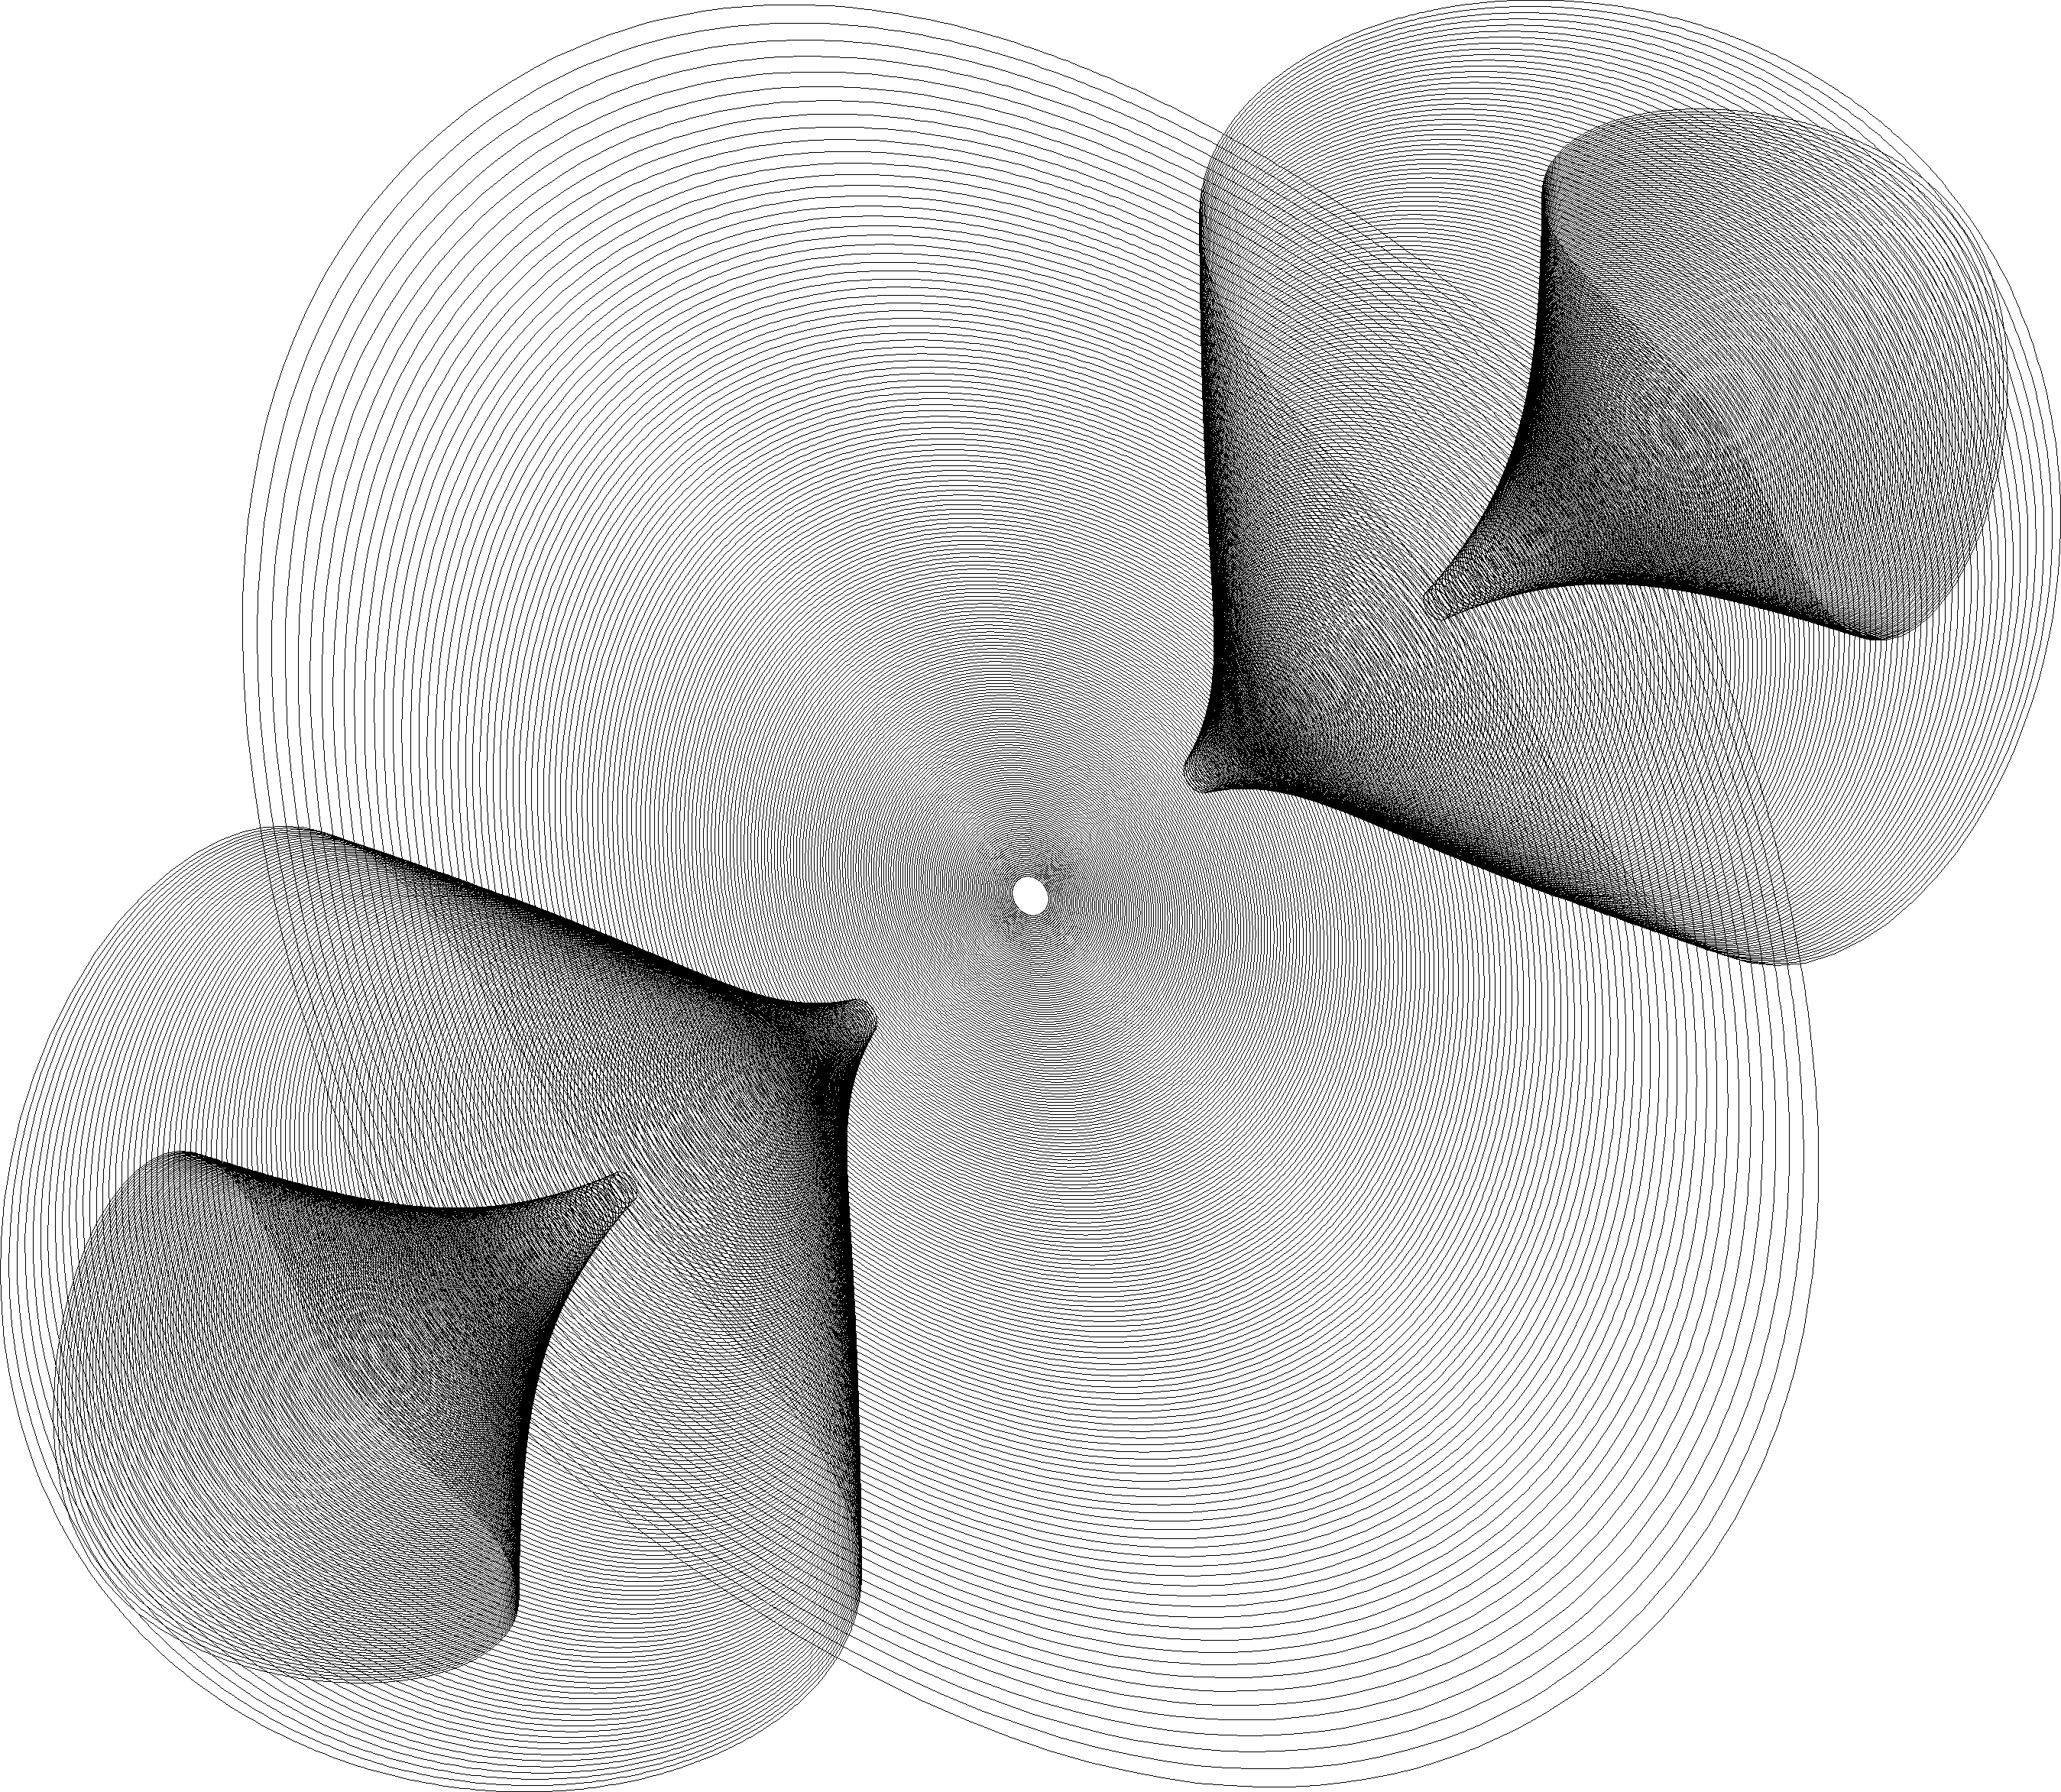
\includegraphics[height=8cm]{graphics/moduli_plot_p1.png}
\end{center}
\end{frame}

\begin{frame}
\begin{center}
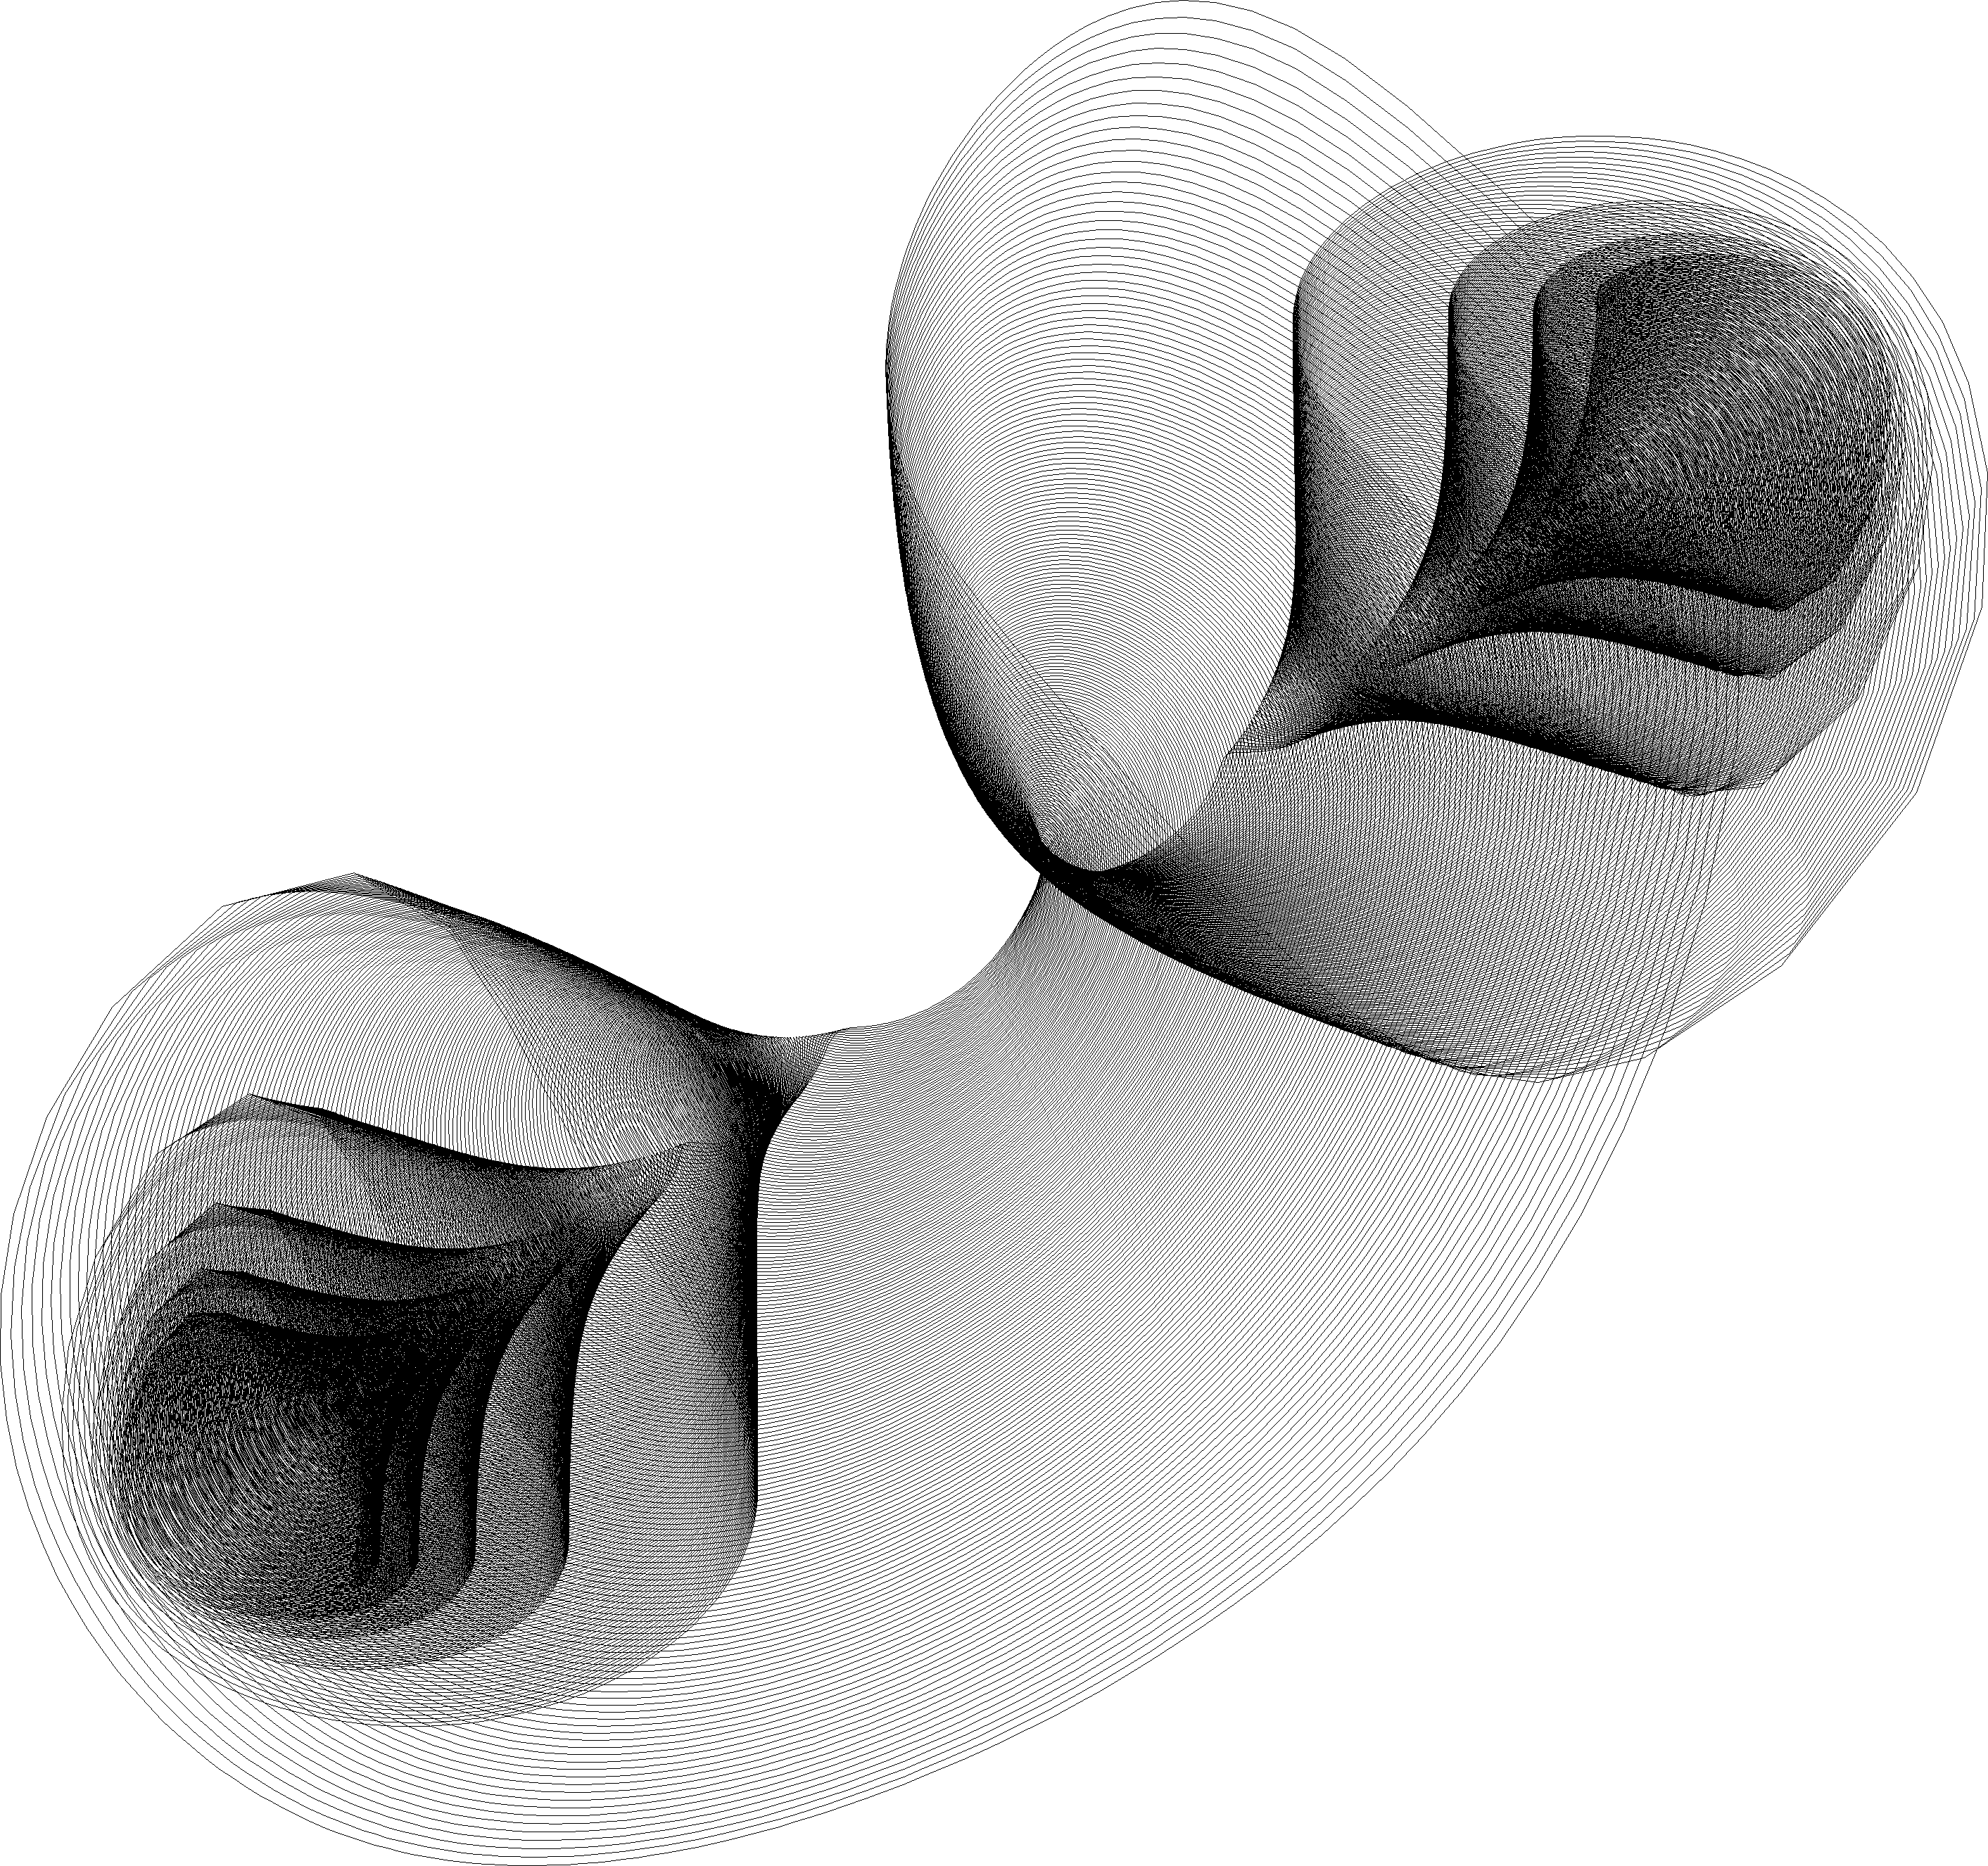
\includegraphics[height=9cm]{graphics/moduli_plot_p2.png}
\end{center}
\end{frame}

\begin{frame}{Method of Proof}
\begin{itemize}
\item Move to the universal cover of the parameter space 
\begin{align*}
π_p : \tilde{\mathcal{A}}_1(p) \to \mathcal{A}_1(p).
\end{align*}
\item Define a function $\tilde{T}$ on $\tilde{\mathcal{A}}_1(p)$ such that $\tilde{T} = T \circ π_p$.
\item In the right coordinates, the level sets of $\tilde{T}$ are graphs over $(0,1)\times\R$.
\item Quotient by deck transformations to recover space of spectral curves.
\item Consider how the lattice of differentials change as you change the spectral curve.
\end{itemize}
\end{frame}


\begin{frame}{Interior Boundary $\mathcal{M}_1$}
\begin{itemize}
\item $\mathcal{M}_1 \cap \mathcal{A}_1(p)$ spirals around the diagonal line $\{α = β\} \cap \mathcal{A}_1(p)$.
\item Just a single point on this diagonal line is reachable along a finite path.
\item This limit seems not to be well-defined.
\end{itemize}
\end{frame}


\begin{frame}{Exterior Boundary $\mathcal{M}_1$}
\begin{itemize}
\item This boundary is where $α$ or $β$ tends to $\S^1$.
\item A singular curve with a double point over the unit circle corresponds to genus zero spectral data via normalisation (blow-up).
\item We can consider $\mathcal{M}_0 \subset \partial \mathcal{M}_1$.
\item Each face of the football $\overline{\mathcal{A}_1(p)}$ is a disc, identified with the space of genus zero spectral curves. 
\item Edges of $\overline{\mathcal{A}_1(p)}$ correspond to all branch points on unit circle, ie a map to a circle.
\end{itemize}
\end{frame}


\begin{frame}{Further questions}
\begin{itemize}
\item Can we identify geometric properties that parameterise $\mathcal{M}$?
\item Is $\mathcal{M}_0 \cup \mathcal{M}_1$ connected? No.
What other maps need to be included to make it connected? 
% \item Are there points in every component of $\mathcal{M}_g$ where all branch points tend to the unit circle?
\item Can one deform a harmonic map to a circle to a harmonic map of any spectral degree?
\item How does $\mathcal{M}_g$ sit inside the moduli space of harmonic cylinders? Harmonic planes?
\item What deformations lead to topological changes of the image of the harmonic map?
\end{itemize}
\end{frame}


\end{document}
